\documentclass[12pt,a4paper]{article}

% ================= PAQUETES =================
\usepackage[utf8]{inputenc}
\usepackage[T1]{fontenc}
\usepackage{newtxtext,newtxmath}
\usepackage[top=2.5cm, bottom=2.5cm, left=3.5cm, right=2.5cm]{geometry}
\usepackage{setspace}
\doublespacing
\usepackage{graphicx}
\usepackage{indentfirst}
\usepackage[hidelinks]{hyperref}
\usepackage{titlesec}
\usepackage{caption}
\usepackage{booktabs}
\usepackage{multirow}
\usepackage{array}
\usepackage{enumitem}
\usepackage{amsmath}
\usepackage{longtable}
\usepackage{float}
\usepackage{tabularx}

% ================= COLORES PARA TABLAS =================
\usepackage[table]{xcolor}

% ================= ALGORITMOS Y PSEUDOCÓDIGO =================
\usepackage[ruled,vlined,onelanguage]{algorithm2e}
\SetKwComment{Comment}{// }{}
\SetKwInput{KwInput}{Entrada}
\SetKwInput{KwOutput}{Salida}
\SetKwFor{ForEach}{para cada}{hacer}{fin para}
\SetKwIF{Si}{SinoSi}{Sino}{si}{entonces}{sino si}{sino}{fin si}
\SetKwFor{Para}{para}{hacer}{fin para}
\SetKwFor{While}{mientras}{hacer}{fin mientras}
\SetKwProg{Fn}{Función}{:}{fin}

% ================= SUBFIGURAS =================
\usepackage{subcaption}

% ================= FORMATO DE TÍTULOS =================
\titleformat{\section}{\normalfont\Large\bfseries\centering}{\thesection.}{1em}{\MakeUppercase}
\titleformat{\subsection}{\normalfont\large\bfseries}{\thesubsection.}{1em}{\MakeUppercase}
\titleformat{\subsubsection}{\normalfont\normalsize\bfseries}{\thesubsubsection.}{1em}{}

% ================= FORMATO DE TABLAS Y FIGURAS =================
\captionsetup[table]{labelsep=newline, textfont=it, font=normalsize, justification=raggedright, singlelinecheck=off}
\captionsetup[figure]{labelsep=newline, textfont=it, font=normalsize, justification=raggedright, singlelinecheck=off}

% ================= PÁRRAFOS =================
\setlength{\parindent}{1.25cm}
\setlength{\parskip}{10pt}

\usepackage[spanish,es-tabla]{babel}

\begin{document}
\thispagestyle{empty}
\begin{center}
    {\fontsize{18}{21}\selectfont \textbf{UNIVERSIDAD NACIONAL DEL ALTIPLANO} \par}
    \vspace{0.3cm}
    {\fontsize{14}{17}\selectfont \textbf{Árboles de Dependencia, Información Mutua y Redes Bayesianas} \par}
    \vspace{0.3cm}
    {\fontsize{14}{17}\selectfont \textbf{Predicción de Abandono Universitario} \par}
    \vspace{0.5cm}
    {\fontsize{12}{15}\selectfont JAHUIRA PONCE CHRISTIAN SEBASTIÁN \par}
    \vspace{0.3cm}
    {\fontsize{12}{15}\selectfont PUNO -- PERÚ -- 2026 \par}
\end{center}
\newpage
\section{Dataset B -- Desplazados (2,426 registros)}

\subsection{Desarrollo de Entropía}

La entropía general es menor en este grupo, reflejando un perfil más homogéneo.

\subsubsection{Cálculo para $x_1$ (Nota de admisión)}
Probabilidades: $p(0) = \frac{741}{2426} = 0.3054$, $p(1) = \frac{852}{2426} = 0.3512$, $p(2) = \frac{833}{2426} = 0.3434$
\begin{align*}
    H(x_1) &= -\big[ (0.3054 \cdot \log_2(0.3054)) + (0.3512 \cdot \log_2(0.3512)) + (0.3434 \cdot \log_2(0.3434)) \big] \\
    H(x_1) &= 0.5227 + 0.5298 + 0.5286 = \textbf{1.5801}
\end{align*}

\subsubsection{Cálculo para $x_2$ (Edad)}
Probabilidades: $p(0) = \frac{1228}{2426} = 0.5062$, $p(1) = \frac{584}{2426} = 0.2407$, $p(2) = \frac{614}{2426} = 0.2531$
\begin{align*}
    H(x_2) &= -\big[ (0.5062 \cdot \log_2(0.5062)) + (0.2407 \cdot \log_2(0.2407)) + (0.2531 \cdot \log_2(0.2531)) \big] \\
    H(x_2) &= 0.4976 + 0.4937 + 0.5032 = \textbf{1.3999}
\end{align*}

\subsubsection{Cálculo para $x_3$ (Pagos al día)}
Probabilidades: $p(0) = \frac{269}{2426} = 0.1109$, $p(1) = \frac{2157}{2426} = 0.8891$
\begin{align*}
    H(x_3) &= -\left[ (0.1109 \cdot \log_2(0.1109)) + (0.8891 \cdot \log_2(0.8891)) \right] \\
    H(x_3) &= 0.3522 + 0.1505 = \textbf{0.4401}
\end{align*}

\subsubsection{Cálculo para $x_4$ (Becado)}
Probabilidades: $p(0) = \frac{1935}{2426} = 0.7976$, $p(1) = \frac{491}{2426} = 0.2024$
\begin{align*}
    H(x_4) &= -\left[ (0.7976 \cdot \log_2(0.7976)) + (0.2024 \cdot \log_2(0.2024)) \right] \\
    H(x_4) &= 0.2605 + 0.4665 = \textbf{0.8513}
\end{align*}

\subsubsection{Cálculo para $x_5$ (1er sem. aprobados)}
Probabilidades: $p(0) = \frac{927}{2426} = 0.3821$, $p(1) = \frac{1067}{2426} = 0.4398$, $p(2) = \frac{432}{2426} = 0.1781$
\begin{align*}
    H(x_5) &= 0.5310 + 0.5219 + 0.4436 = \textbf{1.5102}
\end{align*}

\subsubsection{Cálculo para $x_6$ (1er sem. nota)}
Probabilidades: $p(0) = \frac{807}{2426} = 0.3326$, $p(1) = \frac{887}{2426} = 0.3656$, $p(2) = \frac{732}{2426} = 0.3017$
\begin{align*}
    H(x_6) &= 0.5290 + 0.5302 + 0.5215 = \textbf{1.5790}
\end{align*}

\subsubsection{Cálculo para $x_7$ (2do sem. aprobados)}
Probabilidades: $p(0) = \frac{947}{2426} = 0.3904$, $p(1) = \frac{980}{2426} = 0.4040$, $p(2) = \frac{499}{2426} = 0.2057$
\begin{align*}
    H(x_7) &= 0.5294 + 0.5281 + 0.4698 = \textbf{1.5273}
\end{align*}

\subsubsection{Cálculo para $x_8$ (2do sem. nota)}
Probabilidades: $p(0) = \frac{805}{2426} = 0.3318$, $p(1) = \frac{909}{2426} = 0.3747$, $p(2) = \frac{712}{2426} = 0.2935$
\begin{align*}
    H(x_8) &= 0.5286 + 0.5303 + 0.5223 = \textbf{1.5812}
\end{align*}

\subsubsection{Cálculo para $x_9$ (Estado civil)}
Probabilidades: $p(0) = \frac{2254}{2426} = 0.9291$, $p(1) = \frac{172}{2426} = 0.0709$
\begin{align*}
    H(x_9) &= -\left[ (0.9291 \cdot \log_2(0.9291)) + (0.0709 \cdot \log_2(0.0709)) \right] \\
    H(x_9) &= 0.0986 + 0.2707 = \textbf{0.2171}
\end{align*}

\subsubsection{Cálculo para Target}
Probabilidades: $p(0) = \frac{669}{2426} = 0.2758$, $p(1) = \frac{433}{2426} = 0.1785$, $p(2) = \frac{1324}{2426} = 0.5458$
\begin{align*}
    H(Target) &= 0.5124 + 0.4432 + 0.4775 = \textbf{1.4331}
\end{align*}

\subsection{Matriz de Información Mutua}

\subsubsection{Ejemplo detallado: $x_5$ con $x_7$}
Probabilidades conjuntas principales y sus términos:

\begin{align*}
    \text{Term. } (0,0) &= 0.3199 \cdot \log_2\left(\frac{0.3199}{0.3821 \cdot 0.3904}\right) = 0.3199 \cdot \log_2(2.1458) = \mathbf{+0.3521} \\
    \text{Term. } (1,1) &= 0.3293 \cdot \log_2\left(\frac{0.3293}{0.4398 \cdot 0.4040}\right) = 0.3293 \cdot \log_2(1.8530) = \mathbf{+0.2929} \\
    \text{Term. } (2,2) &= 0.1311 \cdot \log_2\left(\frac{0.1311}{0.1781 \cdot 0.2057}\right) = 0.1311 \cdot \log_2(3.5808) = \mathbf{+0.2406}
\end{align*}
\textbf{Suma Total:} $IM(x_5, x_7) = \textbf{0.8335}$ (incluyendo términos cruzados negativos)

\subsubsection{Matriz Resultante (10$\times$10)}

\begin{table}[H]
    \centering
    \footnotesize
    \begin{tabular}{c|cccccccccc}
        \toprule
        & $\mathbf{x_1}$ & $\mathbf{x_2}$ & $\mathbf{x_3}$ & $\mathbf{x_4}$ & $\mathbf{x_5}$ & $\mathbf{x_6}$ & $\mathbf{x_7}$ & $\mathbf{x_8}$ & $\mathbf{x_9}$ & \textbf{Target} \\
        \midrule
        $\mathbf{x_1}$ & 0 & 0.0305 & 0.0061 & 0.0037 & 0.0116 & 0.0307 & 0.0139 & 0.0231 & 0.0028 & 0.0106 \\
        $\mathbf{x_2}$ & 0.0305 & 0 & 0.0158 & 0.0277 & 0.0261 & 0.0231 & 0.0251 & 0.0213 & 0.0782 & 0.0467 \\
        $\mathbf{x_3}$ & 0.0061 & 0.0158 & 0 & 0.0121 & 0.0356 & 0.0312 & 0.0491 & 0.0451 & 0.0002 & 0.0992 \\
        $\mathbf{x_4}$ & 0.0037 & 0.0277 & 0.0121 & 0 & 0.0347 & 0.0263 & 0.0482 & 0.0255 & 0.0070 & 0.0585 \\
        $\mathbf{x_5}$ & 0.0116 & 0.0261 & 0.0356 & 0.0347 & 0 & 0.2954 & \textbf{0.8335} & 0.3204 & 0.0062 & 0.2331 \\
        $\mathbf{x_6}$ & 0.0307 & 0.0231 & 0.0312 & 0.0263 & 0.2954 & 0 & 0.2955 & \textbf{0.4695} & 0.0068 & 0.1562 \\
        $\mathbf{x_7}$ & 0.0139 & 0.0251 & 0.0491 & 0.0482 & \textbf{0.8335} & 0.2955 & 0 & 0.3632 & 0.0049 & 0.2964 \\
        $\mathbf{x_8}$ & 0.0231 & 0.0213 & 0.0451 & 0.0255 & 0.3204 & \textbf{0.4695} & 0.3632 & 0 & 0.0052 & 0.2226 \\
        $\mathbf{x_9}$ & 0.0028 & \textbf{0.0782} & 0.0002 & 0.0070 & 0.0062 & 0.0068 & 0.0049 & 0.0052 & 0 & 0.0071 \\
        \textbf{Target} & 0.0106 & 0.0467 & 0.0992 & 0.0585 & 0.2331 & 0.1562 & \textbf{0.2964} & 0.2226 & 0.0071 & 0 \\
        \bottomrule
    \end{tabular}
    \caption{Matriz de Información Mutua -- Dataset B.}
\end{table}

\subsection{Algoritmo de Kruskal (MST)}

\begin{enumerate}[label=\textbf{\arabic*.}]
    \item $x_5 - x_7$ (Peso: 0.8335) $\rightarrow$ \textbf{Aceptado}
    \item $x_6 - x_8$ (Peso: 0.4695) $\rightarrow$ \textbf{Aceptado}
    \item $x_7 - x_8$ (Peso: 0.3632) $\rightarrow$ \textbf{Aceptado}
    \item $x_6 - x_5$ (Peso: 0.2954) $\rightarrow$ \textbf{Rechazado} (Ciclo con $x_5$, $x_7$, $x_8$)
    \item $x_7 - Target$ (Peso: 0.2964) $\rightarrow$ \textbf{Aceptado}
    \item $x_2 - x_9$ (Peso: 0.0782) $\rightarrow$ \textbf{Aceptado}
    \item $x_3 - Target$ (Peso: 0.0992) $\rightarrow$ \textbf{Aceptado}
    \item $x_4 - Target$ (Peso: 0.0585) $\rightarrow$ \textbf{Aceptado}
    \item $x_2 - Target$ (Peso: 0.0467) $\rightarrow$ \textbf{Aceptado}
    \item $x_1 - x_6$ (Peso: 0.0307) $\rightarrow$ \textbf{Aceptado} (Última arista)
\end{enumerate}

\textbf{Cálculo del Peso del MST (Dataset B):}
\begin{equation}
    MST_B = 0.8335 + 0.4695 + 0.3632 + 0.2964 + 0.0782 + 0.0992 + 0.0585 + 0.0467 + 0.0307 = \textbf{2.2759}
\end{equation}

\subsection{Validación por Algoritmo de Prim}
Partiendo del nodo Target:

\begin{itemize}
    \item \textbf{Paso 1:} Desde Target $\rightarrow$ Mayor: \textbf{$x_7$} (0.2964).
    \item \textbf{Paso 2:} Desde $x_7$ $\rightarrow$ Mayor: \textbf{$x_5$} (0.8335).
    \item \textbf{Paso 3:} Desde $x_7$ $\rightarrow$ Mayor libre: \textbf{$x_8$} (0.3632).
    \item \textbf{Paso 4:} Desde $x_8$ $\rightarrow$ Mayor: \textbf{$x_6$} (0.4695).
    \item \textbf{Paso 5:} Desde Target $\rightarrow$ Mayor libre: \textbf{$x_3$} (0.0992).
    \item \textbf{Paso 6:} Desde Target $\rightarrow$ Mayor libre: \textbf{$x_4$} (0.0585).
    \item \textbf{Paso 7:} Desde Target $\rightarrow$ Mayor libre: \textbf{$x_2$} (0.0467).
    \item \textbf{Paso 8:} Desde $x_2$ $\rightarrow$ Mayor libre: \textbf{$x_9$} (0.0782).
    \item \textbf{Paso 9:} Desde $x_6$ $\rightarrow$ Mayor libre: \textbf{$x_1$} (0.0307).
\end{itemize}

Prim genera las mismas 9 aristas, confirmando un MST de peso \textbf{2.2759}.

\subsection{Árbol de Dependencias}

\begin{figure}[H]
    \centering
    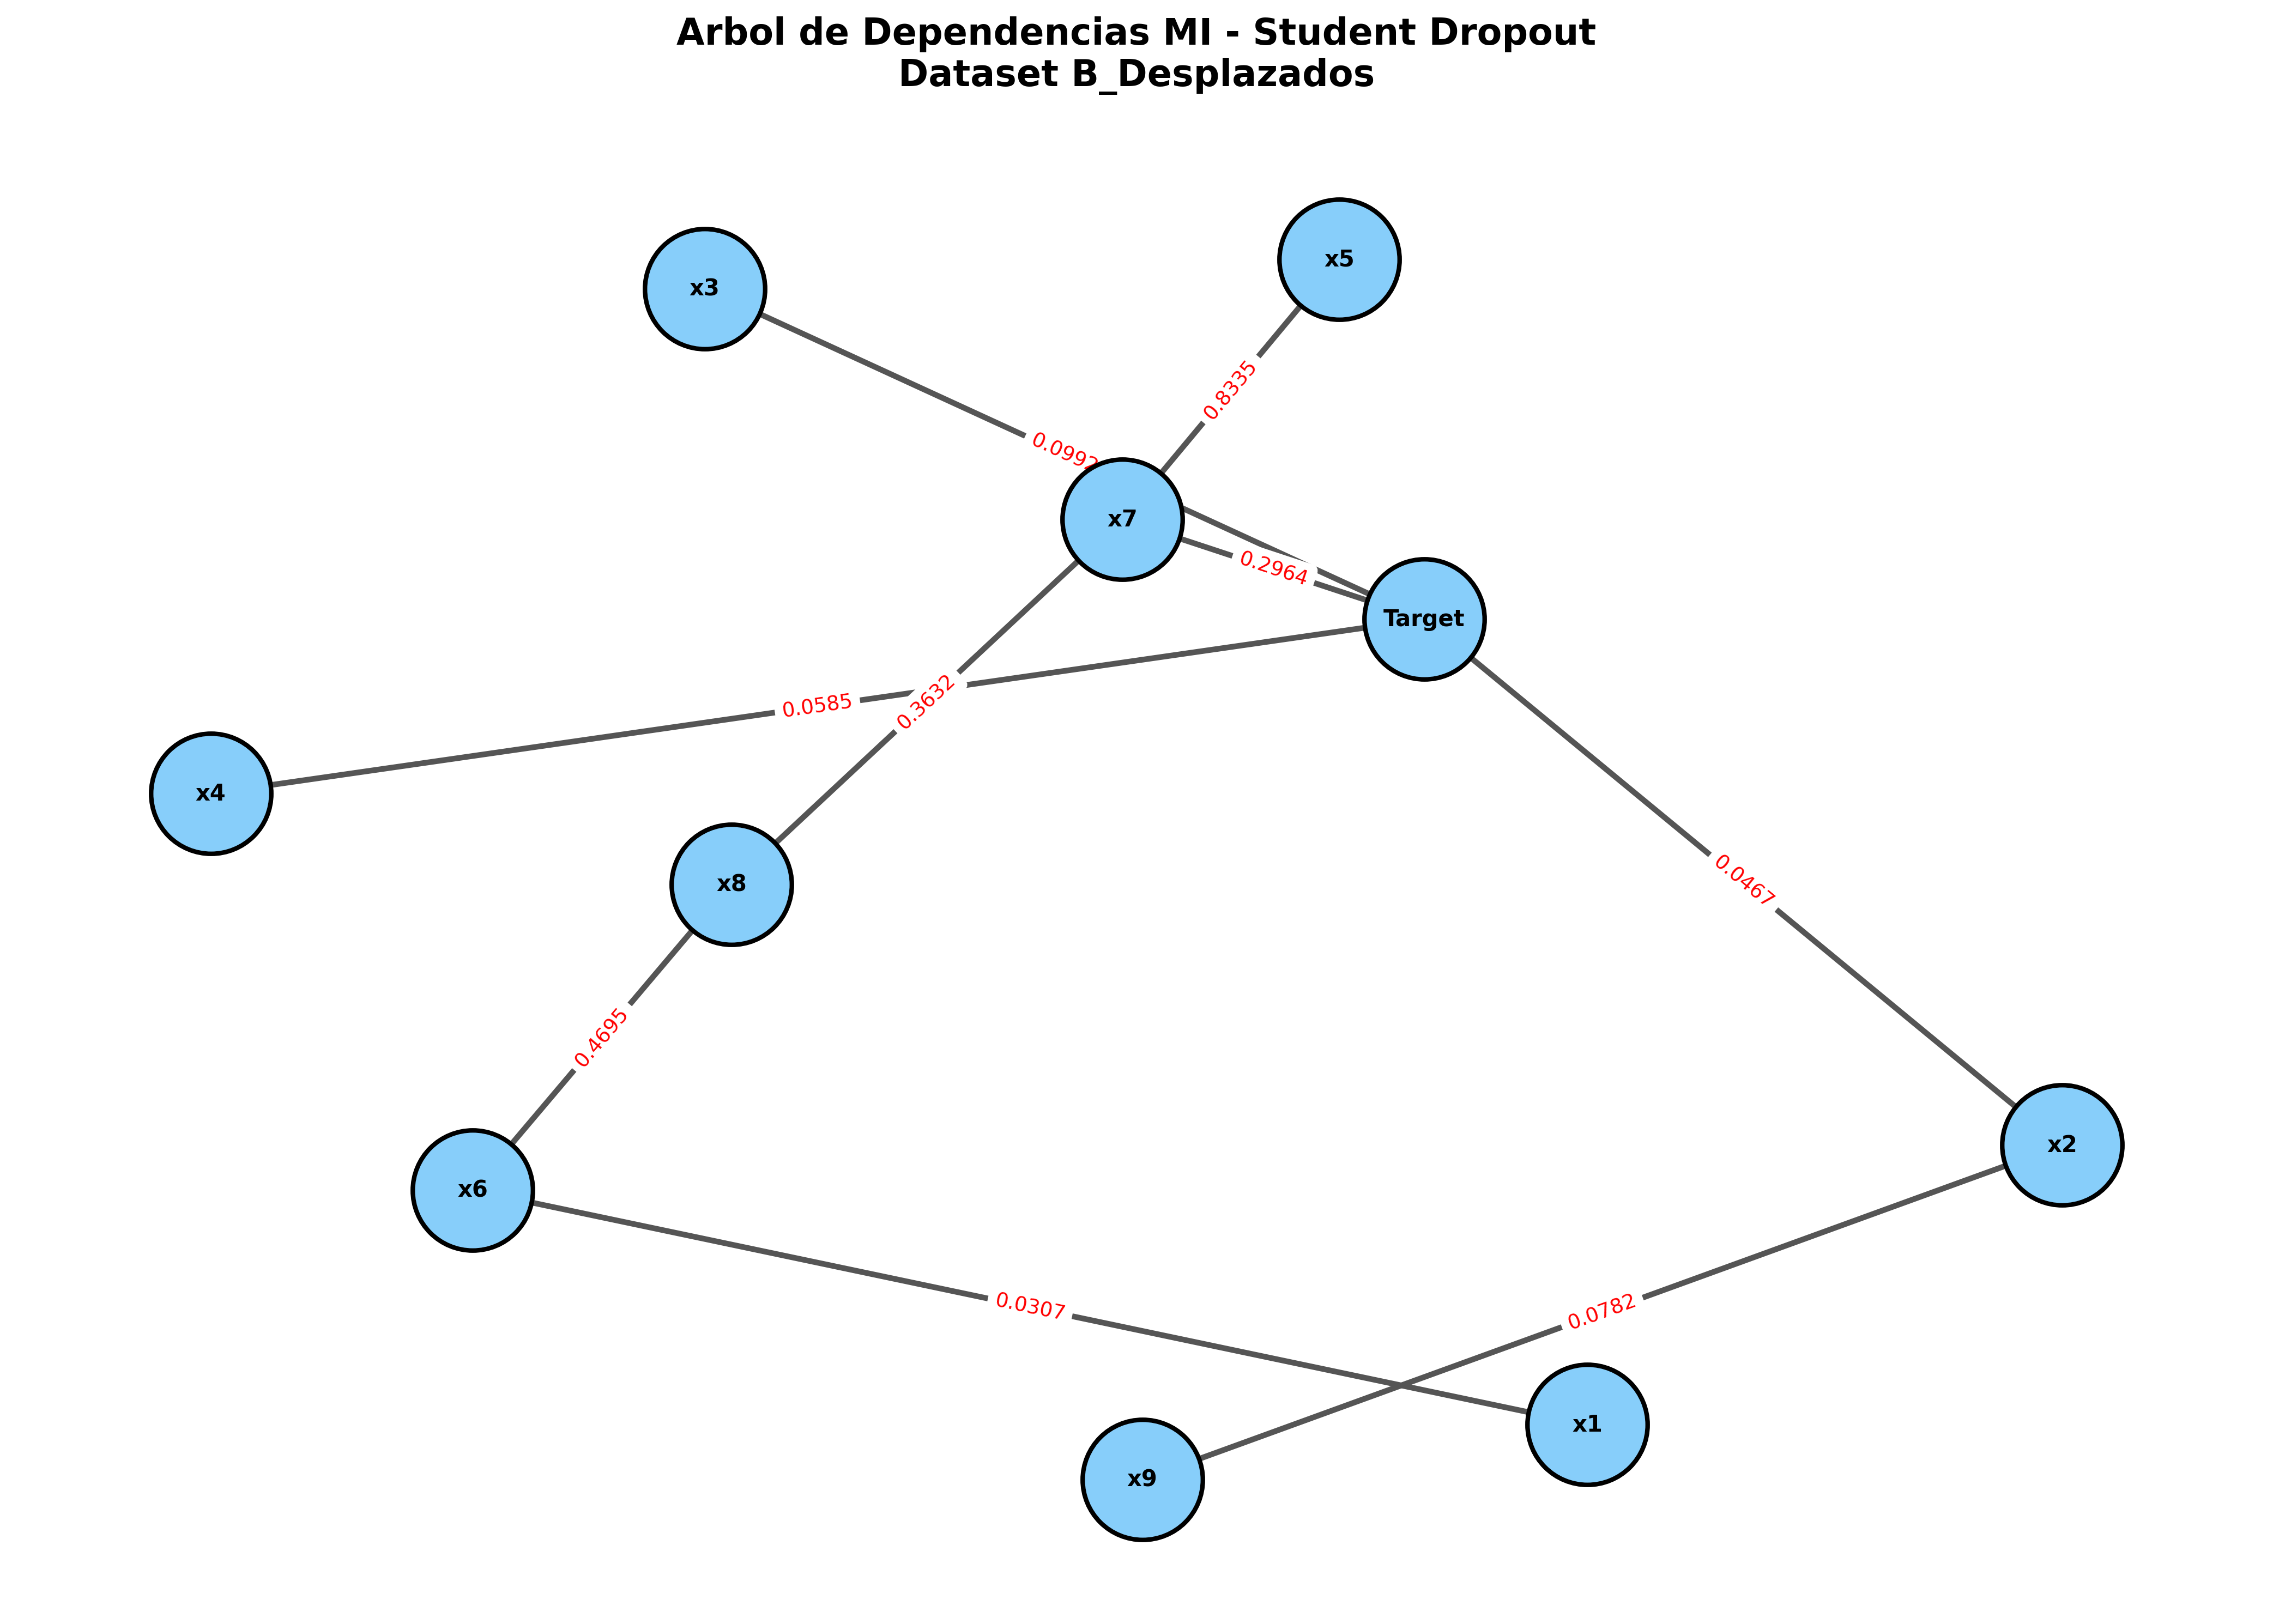
\includegraphics[width=0.85\textwidth]{arbol_B_Desplazados.png}
    \caption{Árbol de Expansión Máxima -- Dataset B (Desplazados).}
    \label{fig:arbolB}
\end{figure}

\begin{figure}[H]
    \centering
    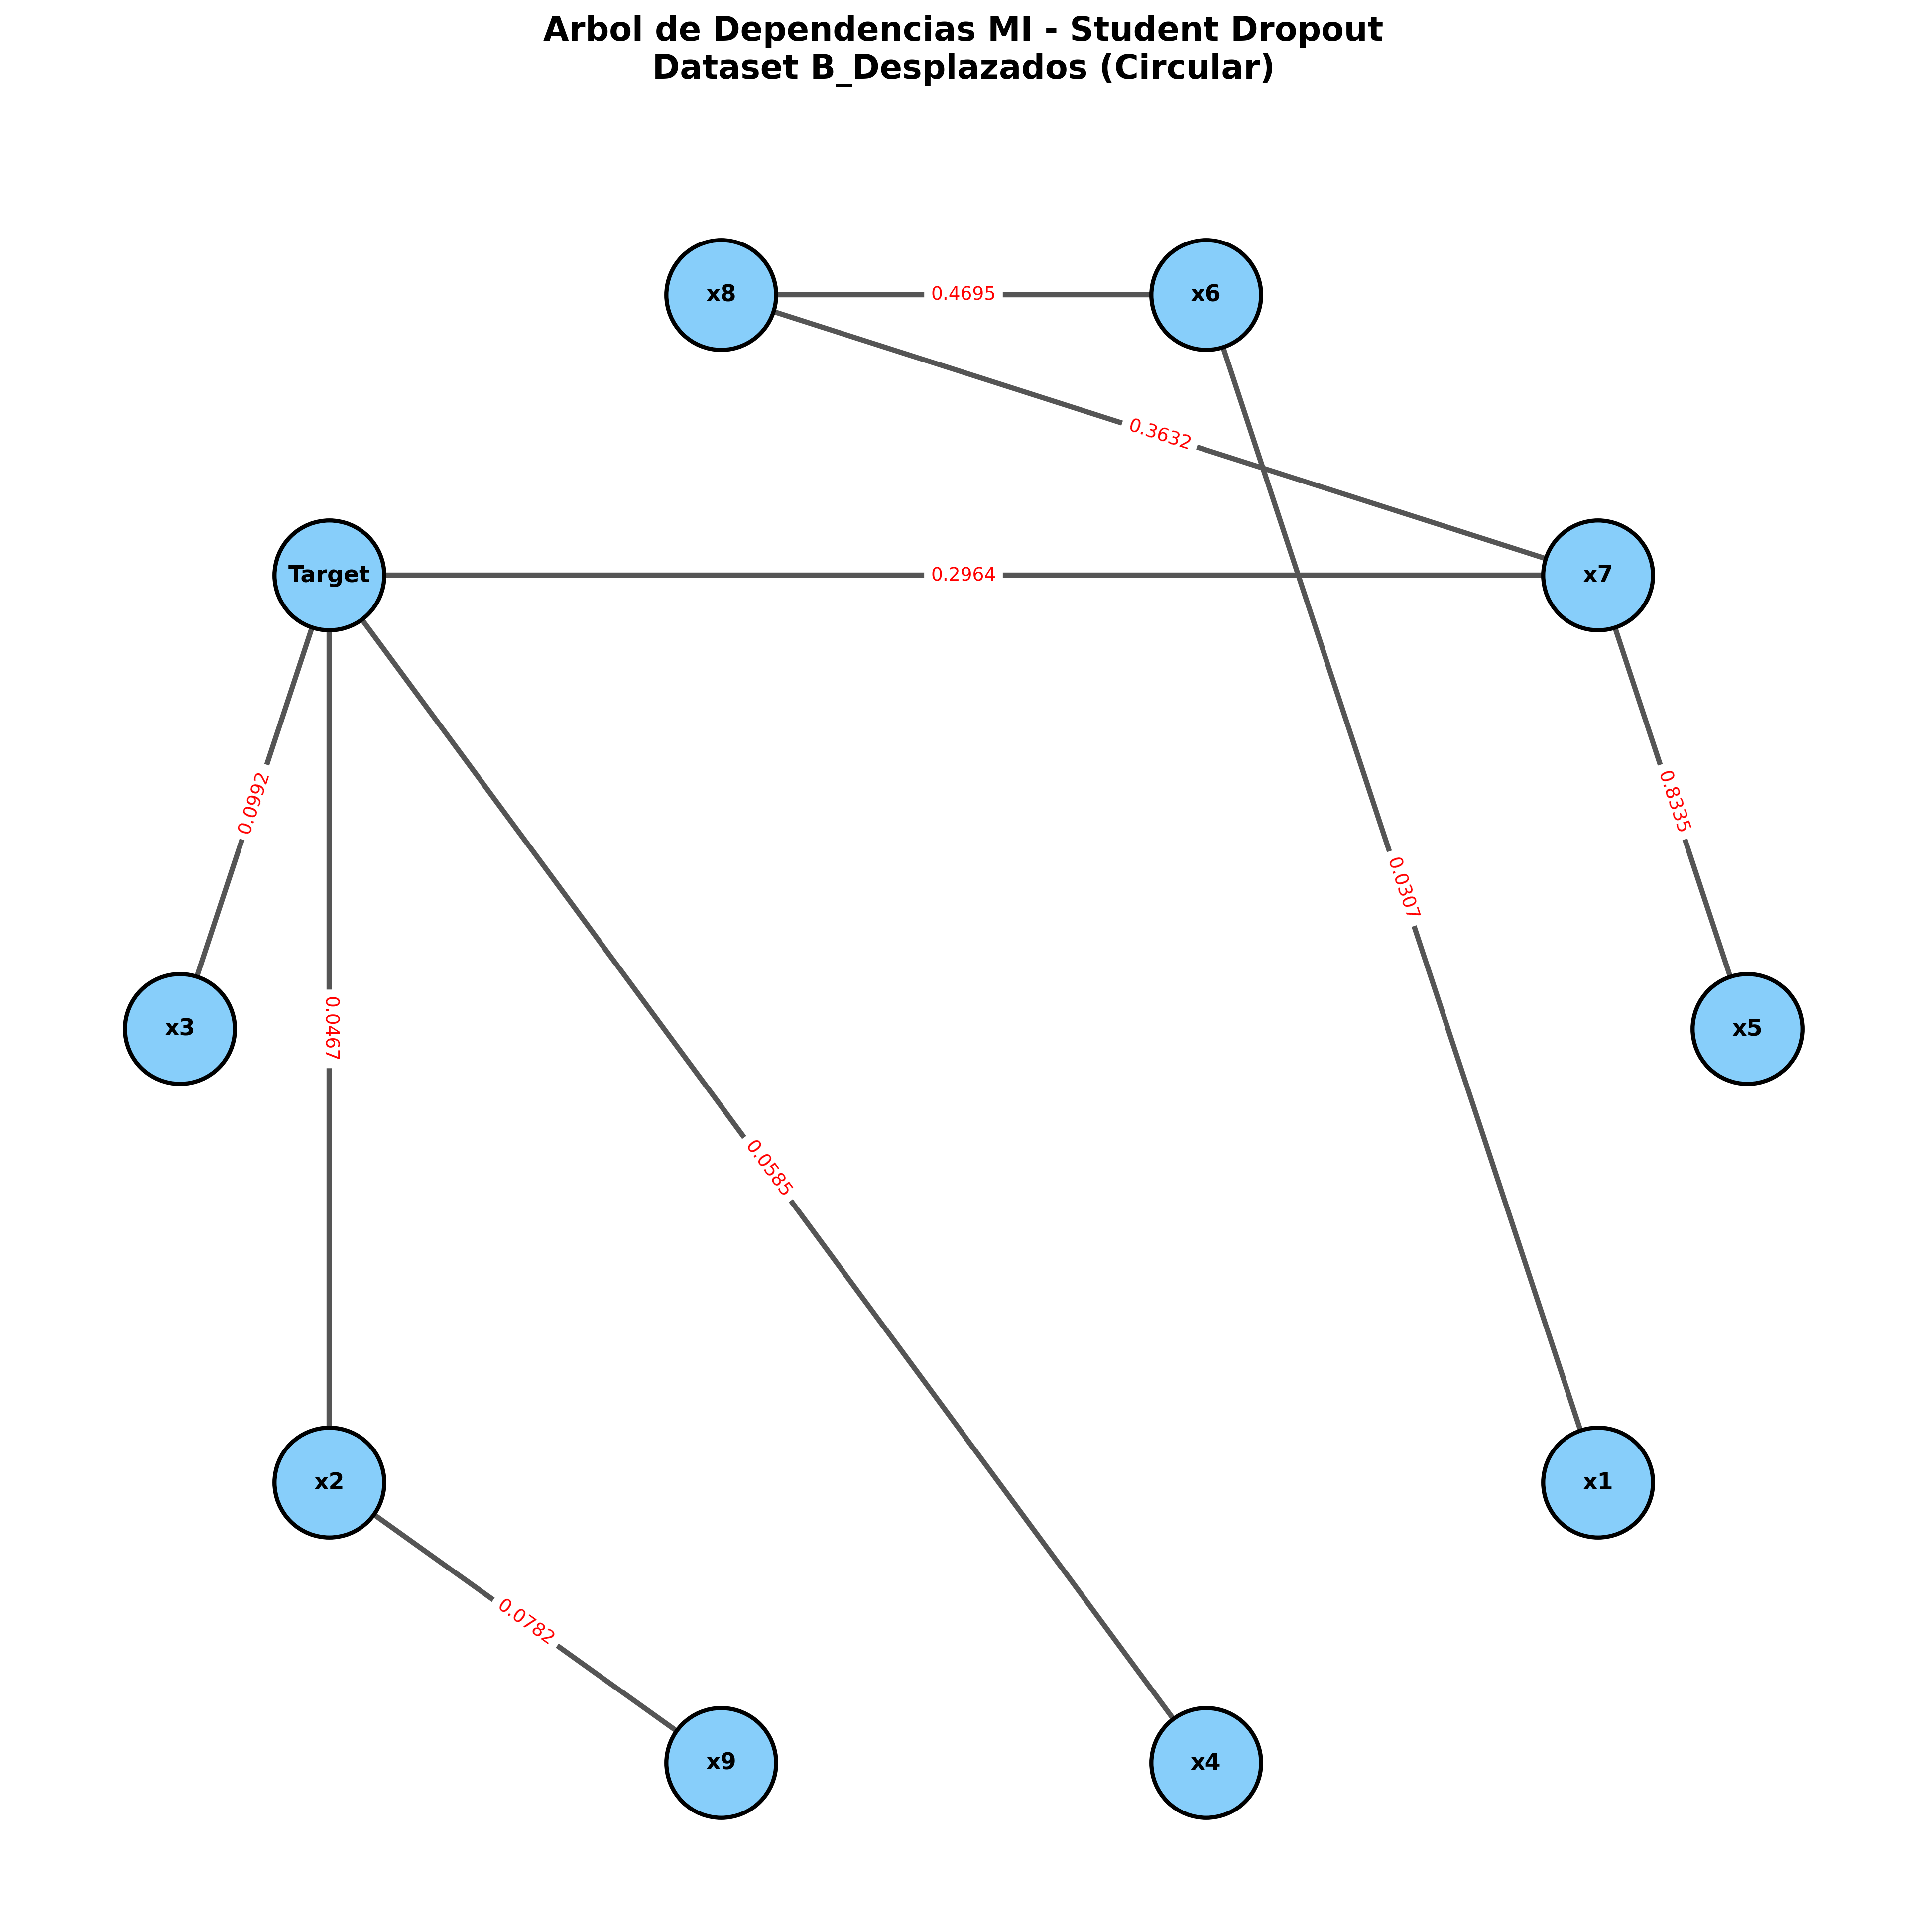
\includegraphics[width=0.75\textwidth]{arbol_B_Desplazados_circular.png}
    \caption{Distribución Circular del Árbol -- Dataset B (Desplazados).}
    \label{fig:arbolB_circ}
\end{figure}

% =============================================
% COMPARATIVA Y ANÁLISIS
% =============================================
\newpage
\section{Análisis Comparativo}

\subsection{Comparativa de Entropías}

\begin{table}[H]
    \centering
    \begin{tabular}{c|ccc}
        \toprule
        \textbf{Variable} & $H(A)$ & $H(B)$ & $H(Original)$ \\
        \midrule
        $x_1$ (Nota admisión) & 1.5773 & 1.5801 & 1.5850 \\
        $x_2$ (Edad) & 1.4795 & 1.3999 & 1.5435 \\
        $x_3$ (Pagos al día) & 0.6189 & 0.4401 & 0.5275 \\
        $x_4$ (Becado) & 0.7485 & 0.8513 & 0.8088 \\
        $x_5$ (1sem aprobados) & 1.4897 & 1.5102 & 1.5055 \\
        $x_6$ (1sem nota) & 1.5724 & 1.5790 & 1.5840 \\
        $x_7$ (2sem aprobados) & 1.4851 & 1.5273 & 1.5126 \\
        $x_8$ (2sem nota) & 1.5754 & 1.5812 & 1.5824 \\
        $x_9$ (Estado civil) & 0.7428 & 0.2171 & 0.5123 \\
        \midrule
        Target & 1.4970 & 1.4331 & 1.4713 \\
        \bottomrule
    \end{tabular}
    \caption{Comparativa de entropías entre datasets.}
\end{table}

\textbf{Observación sobre $x_9$ (Estado civil):} En el dataset original, el estado civil tiene una entropía moderada ($H = 0.5123$) con distribución $88.6\%$ solteros y $11.4\%$ otros. Al particionar por desplazamiento, el Dataset A presenta $H_A = 0.7428$, mientras que el Dataset B colapsa a $H_B = 0.2171$. Esto evidencia que los estudiantes desplazados son casi en su totalidad solteros ($92.9\%$), mientras que los no desplazados tienen mayor diversidad de estados civiles.

\subsection{Comparativa de Árboles MST}

\begin{table}[H]
    \centering
    \begin{tabular}{c|c|c}
        \toprule
        & \textbf{Dataset A (No Desp)} & \textbf{Dataset B (Desp)} \\
        \midrule
        Arista 1 & $x_5 - x_7$ (0.7209) & $x_5 - x_7$ (0.8335) \\
        Arista 2 & $x_6 - x_8$ (0.3754) & $x_6 - x_8$ (0.4695) \\
        Arista 3 & $x_7 - Target$ (0.3760) & $x_7 - x_8$ (0.3632) \\
        Arista 4 & $x_7 - x_8$ (0.3094) & $x_7 - Target$ (0.2964) \\
        Arista 5 & $x_2 - x_9$ (0.1958) & $x_2 - x_9$ (0.0782) \\
        Arista 6 & $x_3 - Target$ (0.1643) & $x_3 - Target$ (0.0992) \\
        Arista 7 & $x_4 - Target$ (0.0839) & $x_4 - Target$ (0.0585) \\
        Arista 8 & $x_2 - Target$ (0.0828) & $x_2 - Target$ (0.0467) \\
        Arista 9 & $x_1 - x_6$ (0.0336) & $x_1 - x_6$ (0.0307) \\
        \midrule
        \rowcolor{blue!15}
        Peso total & \textbf{2.3421} & \textbf{2.2759} \\
        \bottomrule
    \end{tabular}
    \caption{Comparativa de aristas del MST.}
\end{table}

\textbf{Hallazgos principales:}
\begin{itemize}
    \item Ambos datasets conservan una estructura muy similar: el \textbf{bloque académico} ($x_5$, $x_6$, $x_7$, $x_8$) forma el núcleo del árbol, con $x_7$ (2do semestre aprobados) como puente hacia el Target.
    \item La conexión $x_5 - x_7$ es consistentemente la de mayor peso en ambos datasets (0.7209 en A, 0.8335 en B), indicando una fuerte dependencia entre el rendimiento del primer y segundo semestre.
    \item El Target se conecta directamente a 4 variables en ambos datasets: $x_7$ (rendimiento), $x_3$ (pagos), $x_4$ (beca) y $x_2$ (edad), siendo $x_7$ el predictor más fuerte.
    \item Los pesos totales del MST son muy similares (2.3421 vs 2.2759), indicando que la estructura global de dependencias es robusta a la partición por desplazamiento.
    \item $x_1$ (nota de admisión) es consistentemente la variable más periférica, conectada a $x_6$ con pesos bajos en ambos datasets.
\end{itemize}

% =============================================
% ANÁLISIS DE SENSIBILIDAD — rVP
% =============================================
\newpage
\section{Análisis de Sensibilidad -- Método rVP}

\subsection{Matriz de Distancias de Camino}

La distancia de camino $d(x_i, x_j)$ se define como la suma de los pesos de todas las aristas que conforman el camino único entre dos nodos en el MST:

\begin{equation}
    d(x_i, x_j) = \sum_{e \in \text{camino}(x_i \rightarrow x_j)} w(e)
\end{equation}

\subsubsection{Dataset A (No Desplazados)}

\begin{table}[H]
    \centering
    \footnotesize
    \begin{tabular}{c|cccccccccc|c}
        \toprule
        $d(i,j)$ & $\mathbf{x_1}$ & $\mathbf{x_2}$ & $\mathbf{x_3}$ & $\mathbf{x_4}$ & $\mathbf{x_5}$ & $\mathbf{x_6}$ & $\mathbf{x_7}$ & $\mathbf{x_8}$ & $\mathbf{x_9}$ & \textbf{Target} & $\mathbf{\Sigma}$ \\
        \midrule
        $\mathbf{x_1}$   & 0 & 0.4876 & 0.5739 & 0.4935 & 0.7545 & 0.0336 & 0.3786 & 0.3430 & 0.5980 & 0.4424 & 4.1052 \\
        $\mathbf{x_2}$   & 0.4876 & 0 & 0.2471 & 0.1667 & 0.3417 & 0.4540 & 0.0539 & 0.3633 & 0.1958 & 0.0828 & 2.3929 \\
        $\mathbf{x_3}$   & 0.5739 & 0.2471 & 0 & 0.2485 & 0.5525 & 0.5403 & 0.1643 & 0.4737 & 0.4429 & 0.1643 & 3.4074 \\
        $\mathbf{x_4}$   & 0.4935 & 0.1667 & 0.2485 & 0 & 0.4669 & 0.4599 & 0.0839 & 0.3932 & 0.3625 & 0.0839 & 2.7589 \\
        $\mathbf{x_5}$   & 0.7545 & 0.3417 & 0.5525 & 0.4669 & 0 & 0.7545 & 0.7209 & 0.3094 & 0.5375 & 0.3760 & 4.8129 \\
        $\mathbf{x_6}$   & 0.0336 & 0.4540 & 0.5403 & 0.4599 & 0.7545 & 0 & 0.3754 & 0.3754 & 0.5644 & 0.4088 & 3.9660 \\
        $\mathbf{x_7}$   & 0.3786 & 0.0539 & 0.1643 & 0.0839 & 0.7209 & 0.3754 & 0 & 0.3094 & 0.2497 & 0.3760 & 2.7120 \\
        $\mathbf{x_8}$   & 0.3430 & 0.3633 & 0.4737 & 0.3932 & 0.3094 & 0.3754 & 0.3094 & 0 & 0.4737 & 0.6854 & 3.7264 \\
        $\mathbf{x_9}$   & 0.5980 & 0.1958 & 0.4429 & 0.3625 & 0.5375 & 0.5644 & 0.2497 & 0.4737 & 0 & 0.2786 & 3.7030 \\
        \textbf{Target}  & 0.4424 & 0.0828 & 0.1643 & 0.0839 & 0.3760 & 0.4088 & 0.3760 & 0.6854 & 0.2786 & 0 & 2.8981 \\
        \bottomrule
    \end{tabular}
    \caption{Matriz de distancias de caminos -- Dataset A.}
\end{table}

\subsubsection{Dataset B (Desplazados)}

\begin{table}[H]
    \centering
    \footnotesize
    \begin{tabular}{c|cccccccccc|c}
        \toprule
        $d(i,j)$ & $\mathbf{x_1}$ & $\mathbf{x_2}$ & $\mathbf{x_3}$ & $\mathbf{x_4}$ & $\mathbf{x_5}$ & $\mathbf{x_6}$ & $\mathbf{x_7}$ & $\mathbf{x_8}$ & $\mathbf{x_9}$ & \textbf{Target} & $\mathbf{\Sigma}$ \\
        \midrule
        $\mathbf{x_1}$   & 0 & 0.3558 & 0.4754 & 0.4640 & 0.8642 & 0.0307 & 0.3936 & 0.3937 & 0.3990 & 0.4051 & 3.7817 \\
        $\mathbf{x_2}$   & 0.3558 & 0 & 0.1459 & 0.1052 & 0.3542 & 0.3252 & 0.0625 & 0.2945 & 0.0782 & 0.0467 & 1.7682 \\
        $\mathbf{x_3}$   & 0.4754 & 0.1459 & 0 & 0.1577 & 0.4888 & 0.4455 & 0.0992 & 0.4632 & 0.2241 & 0.0992 & 2.5988 \\
        $\mathbf{x_4}$   & 0.4640 & 0.1052 & 0.1577 & 0 & 0.4442 & 0.4339 & 0.0585 & 0.4217 & 0.1834 & 0.0585 & 2.3270 \\
        $\mathbf{x_5}$   & 0.8642 & 0.3542 & 0.4888 & 0.4442 & 0 & 0.8329 & 0.8335 & 0.3632 & 0.3974 & 0.2964 & 4.8748 \\
        $\mathbf{x_6}$   & 0.0307 & 0.3252 & 0.4455 & 0.4339 & 0.8329 & 0 & 0.4695 & 0.4695 & 0.3684 & 0.3758 & 3.7515 \\
        $\mathbf{x_7}$   & 0.3936 & 0.0625 & 0.0992 & 0.0585 & 0.8335 & 0.4695 & 0 & 0.3632 & 0.1407 & 0.2964 & 2.7172 \\
        $\mathbf{x_8}$   & 0.3937 & 0.2945 & 0.4632 & 0.4217 & 0.3632 & 0.4695 & 0.3632 & 0 & 0.3377 & 0.6596 & 3.7665 \\
        $\mathbf{x_9}$   & 0.3990 & 0.0782 & 0.2241 & 0.1834 & 0.3974 & 0.3684 & 0.1407 & 0.3377 & 0 & 0.1249 & 2.2538 \\
        \textbf{Target}  & 0.4051 & 0.0467 & 0.0992 & 0.0585 & 0.2964 & 0.3758 & 0.2964 & 0.6596 & 0.1249 & 0 & 2.3627 \\
        \bottomrule
    \end{tabular}
    \caption{Matriz de distancias de caminos -- Dataset B.}
\end{table}

\subsection{Análisis Diferencial ($\Delta = \Sigma_A - \Sigma_B$)}

\begin{table}[H]
    \centering
    \begin{tabular}{c|ccc|c|c}
        \toprule
        \textbf{Variable} & $\mathbf{\Sigma_A}$ & $\mathbf{\Sigma_B}$ & $\mathbf{\Delta}$ & $\mathbf{|\Delta|}$ & \textbf{¿Crítica?} \\
        \midrule
        $x_1$ (Nota admisión) & 4.1052 & 3.7817 & +0.3235 & 0.3235 & No \\
        $x_2$ (Edad) & 2.3929 & 1.7682 & +0.6247 & 0.6247 & \textbf{Sí} \\
        $x_3$ (Pagos al día) & 3.4074 & 2.5988 & +0.8086 & 0.8086 & \textbf{Sí} \\
        $x_4$ (Becado) & 2.7589 & 2.3270 & +0.4319 & 0.4319 & No \\
        $x_5$ (1sem aprobados) & 4.8129 & 4.8748 & -0.0619 & 0.0619 & No \\
        $x_6$ (1sem nota) & 3.9660 & 3.7515 & +0.2145 & 0.2145 & No \\
        $x_7$ (2sem aprobados) & 2.7120 & 2.7172 & -0.0052 & 0.0052 & No \\
        $x_8$ (2sem nota) & 3.7264 & 3.7665 & -0.0401 & 0.0401 & No \\
        \rowcolor{red!20}
        $x_9$ (Estado civil) & 3.7030 & 2.2538 & \textbf{+1.4492} & 1.4492 & \textbf{Sí} \\
        Target & 2.8981 & 2.3627 & +0.5354 & 0.5354 & \textbf{Sí} \\
        \bottomrule
    \end{tabular}
    \caption{Análisis diferencial rVP (umbral: $|\Delta| > 0.5$).}
\end{table}

\subsection{Variables Críticas}

Con un umbral de $|\Delta| > 0.5$, se identifican 4 variables críticas:

\begin{enumerate}
    \item \textbf{$x_9$ (Estado civil, $\Delta = +1.4492$)}: Es la variable más afectada por la partición. En el Dataset B (desplazados), $x_9$ tiene una entropía mínima ($H_B = 0.2171$) porque el $92.9\%$ de los estudiantes desplazados son solteros. Esto la acerca al centro del árbol en B ($\Sigma_B = 2.25$), mientras que en A está más en la periferia ($\Sigma_A = 3.70$).

    \item \textbf{$x_3$ (Pagos al día, $\Delta = +0.8086$)}: En el Dataset A (no desplazados), $x_3$ está más alejado del centro ($\Sigma_A = 3.41$), mientras que en B se acerca ($\Sigma_B = 2.60$). Esto sugiere que la situación financiera (pagos al día) es más relevante estructuralmente en los estudiantes desplazados.

    \item \textbf{$x_2$ (Edad, $\Delta = +0.6247$)}: Su centralidad varía entre grupos. En B está más cerca del centro ($\Sigma_B = 1.77$), actuando como puente entre $x_9$ y Target, mientras que en A está algo más alejada ($\Sigma_A = 2.39$).

    \item \textbf{Target ($\Delta = +0.5354$)}: La variable objetivo también cambia su posición topológica, estando más integrada al árbol en el Dataset B ($\Sigma_B = 2.36$) que en el A ($\Sigma_A = 2.90$).
\end{enumerate}

\subsection{Conclusiones del Análisis de Sensibilidad}

\begin{itemize}
    \item El \textbf{bloque académico} ($x_5$, $x_6$, $x_7$, $x_8$) muestra una \textbf{robustez estructural notable}: ninguna de estas variables es crítica, indicando que las relaciones de rendimiento académico son estables independientemente del desplazamiento.

    \item \textbf{$x_9$ (estado civil)} emerge como la variable más crítica ($\Delta = +1.4492$). La partición por desplazamiento separa casi perfectamente a los solteros (grupo B) del resto (grupo A), alterando completamente su rol topológico.

    \item Desde la perspectiva del método rVP, la partición por desplazamiento \textbf{afecta principalmente a variables socio-demográficas} ($x_9$, $x_2$) y financieras ($x_3$), mientras que \textbf{el núcleo académico permanece inalterado}. Esto valida que el rendimiento académico es un predictor robusto del abandono universitario, independientemente de la condición de desplazamiento.
\end{itemize}

% =============================================
% REDES BAYESIANAS
% =============================================
\newpage
\end{document}
